
\chapter{Machine learning}
Machine learning is programming computers to optimize a performance
criterion using example data or past experience. In this chapter we present machine learning applications to challenges posed by big data. In Section \ref{BigD}, we give a brief definition of big data  and the challenges currently faced in radio astronomy. In Section \ref{Intro} we give a brief introduction and examples of machine learning,  and in Section \ref{Process}, \ref{comp} we  present the process of machine learning and model complexity.
\section{Big data}
\label{BigD}
\begin{figure}[H]
  \centering
    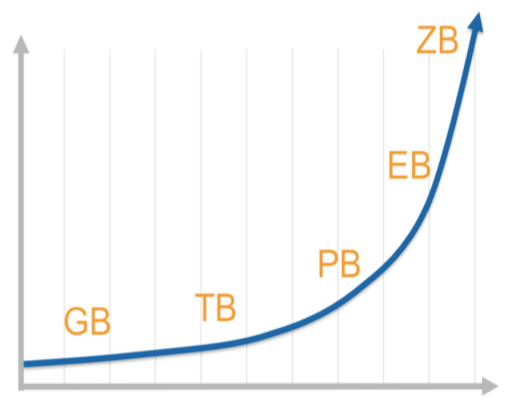
\includegraphics[width=0.5\textwidth]{images/Expgrowth.png}
    \caption{The exponential growth of data from gigabytes to zettabytes [Amazon].}
  \label{datagrowth.png}
\end{figure}
What has changed in the past few decades is the exponential rise in
available computing power, and as a related consequence, the enormous quantities and complexity of the observed data, primarily in digital form.  Such data is refered to as $\textit{big data}$, where traditional data-processing tools are inadequate to deal with them. Big data is now creating, in addition to the natural world, a digital world, in which extracting new and useful information from the data already taken and archived is becoming a major endeavor in itself. This action of knowledge discovery in databases is most commonly inferred by the phrase data mining \citep{ball2010data}. The analogy is that a large volume of earth and raw material is extracted from a mine, which when processed leads to a small
amount of very precious material; similarly, in data mining, a large volume
of data is processed to construct a simple model with valuable use, for example, having high predictive accuracy \citep{alpaydin2014introduction}.



\section{An Introduction to Machine Learning}
\label{Intro}

To solve a problem on a computer, we need an algorithm. An algorithm
is a sequence of instructions that should be carried out to transform
the input to output. e.g, one can design an algorithm for
sorting, where the input is a set of numbers and the output is their ordered
list. For the same task, there may be various algorithms and we may be
interested in finding the most efficient one, requiring the least number of
instructions or memory. For some tasks, however, we do not have an algorithm for example, to tell spam emails from legitimate emails. Therefore what we lack in knowledge, we make up for in data. We can easily compile thousands of example messages some of which we know to be spam and what we want is to "learn" what constitutes spam from them \citep{alpaydin2014introduction}. 

Learning is what gives us flexibility
in our life, the fact that we can adjust and adapt to new circumstances, and learn new
tricks, no mater how old we are. The important parts of human or animal learning is remembering, adapting, and generalising. Being able to recognise late events, and know which actions to be taken, and also knowing how to recognise between different situations, so that things that applied in one place can be used in another is what makes learning useful \citep{marsland2015machine}. 

 Machine learning is not only just a database problem, but also is part
of artificial intelligence. For a system intelligent, it needs to have the ability to learn and adapt in a changing environment. If the system can learn and
adapt to such changes, then it can easily provide predict future solutions without being provided by the system designer \citep{alpaydin2014introduction}. This involves tasks such as recognition, diagnosis,
planning, robot control, prediction, etc \citep{nilsson1996introduction}.
Machine learning also helps us find solutions to many problems in vision,
speech recognition, and robotics. Machine learning is programming computers to optimize a performance criterion using example data or past experience. We have a model defined
up to some parameters, and learning is the execution of a computer program
to optimize the parameters of the model using the training data or
past experience. The model may be predictive to make predictions in the
future, or descriptive to gain knowledge from data.
Machine learning uses the theory of statistics in building mathematical
models, because the core task is making inference from a sample \citep{alpaydin2014introduction}.


Given a class of tasks T, an experience E and measure of performance P. A computer program is said to learn from E with respect to T if the measure P at T improves for more observations E provided \citep{michalski2013machine}. 
\subsection{Examples of Machine learning}
We are surrounded by a machine learning based technology like online shopping where  search engines learn how to bring us the best results and a list of the most relevant products related to our search, email (spam filters, smart email categorization, etc)  where anti-spam software
learns to filter our email messages into spam or not-spam using simple rule filters. Similar approach is used by Gmail to categorize our emails into primary, social, and promotion inboxes, as well as labelling emails as important. 

In a research paper, "The Learning Behind Gmail Priority inbox" \citep{aberdeen2010learning}, google outlines its machine learning approach  and notes " When a user marks messages in a consistent direction, we perform a real-time increment to their threshold". Every time the user mark an email as important, Gmail learns. The researchers tested the effectiveness of Priority Inbox on google employees and found that those with Priority Inbox "spent 6\% less time reading email overall, and 13\% less time reading unimportant email.", social networking (Facebook, etc) where Facebook  automatically highlights faces and suggests friends to tag when uploading a photo. Similar approach is used on digital cameras to learn how to detect faces,  mobile use (Voice to text, smart personal assistants)  where smartphones today are equipped with a standard feature to convert voice-to-text by pressing a button or saying a particular phrase ("Ok Google", for example), you can start speaking and your phone converts the audio into text and recognize voice commands \citep{Techemergence}.  
Machine learning is also widely used in scientific applications such as bioinformatics, medicine, and astronomy.


One common feature of all of these applications is that, in contrast to more
traditional uses of computers, in these cases, due to the complexity of the patterns that need to be detected, a human programmer cannot provide an explicit, fine detailed specification of how such tasks should be executed \citep{shalev2014understanding}. Since in recent years, the world's technology has become increasingly improving as shown in Figure \ref
{datagrowth.png}. This increase led to the amount of data available for learning to dramatically increase. We therefore provide several reasons why machine learning is important given the data challenges.
\begin{itemize}

\item Machine learning methods can often be used to extract the important relationships and correlations of hidden information among "big data". This is also referred to as data mining.

\item The amount of information available about certain tasks might be too large for humans to encode, while as machines can learn this knowledge gradually and be able to capture more of it than humans would \citep{nilsson1996introduction}.

\item Some tasks cannot be defined well except by example; that is, we might be
able to specify input or output pairs but not a concise relationship between
inputs and desired outputs. We would like machines to be able to adjust
their internal structure to produce correct outputs for a large number of
sample inputs and thus suitably constrain their input or output function to
approximate the relationship implicit in the examples \citep{nilsson1996introduction}.
\end{itemize} 

Our focus will be based mainly on tasks that are beyond human capabilities. These are family of tasks that are related to the analysis of very large and complex data sets such as astronomical data. With more and more available digitally recorded data, it becomes obvious that there are treasures of meaningful information buried in data archives that are way too large and too complex for humans
to make sense of. Learning to detect meaningful patterns in large
and complex data sets is a promising domain in which the combination
of programs that learn with the almost unlimited memory
capacity and ever increasing processing speed of computers opens up new horizons \citep{shalev2014understanding}.

\subsection{Types of machine learning}

\begin{figure}[H]
  \centering
    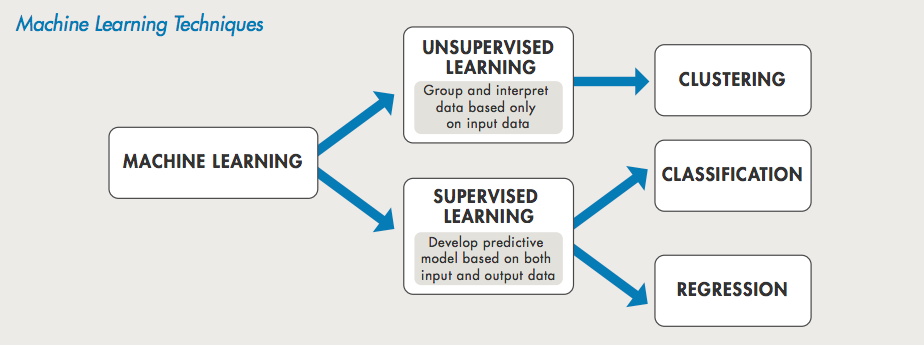
\includegraphics[width=0.7\textwidth]{images/Ml_techs.png}
    \caption{Machine learning techniques include both supervised and unsupervised learning \citep{Machinelearning}.}
  \label{sup-unsup}
\end{figure}

Machine learning algorithms broadly divide into supervised and unsupervised methods, also known as predictive and descriptive, respectively. In supervised learning, the goal is to predict the value of an outcome measure based on a number of input measures as we have an idea about the relationship between the input and output based on the training data set. In contrast to supervised learning, unsupervised learning is in the sense that the data can speak for themselves
without preconceptions such as expected classes being imposed \citep{ball2010data}. 

\subsubsection{Supervised learning}
The aim of supervised machine learning is to build a model
that makes predictions based on evidence in the presence of
uncertainty. Suppose  we want to fit a model $\textbf{Y}=f(\textbf{X})+\epsilon$ with errors $\epsilon$ being additive. Supervised learning attempts to learn the function $f$ by examples given through a teacher. Given the training set with input and output observations $T=(x_i,y_i ), i=1,\dots N$. The observed input values $x_i$ are fed into an artificial system, known as a learning algorithm, which also produces outputs $\widehat{f}(x_i)$ in response to the inputs. The learning algorithm has the property that it can modify its input/output relationship $\widehat{f}$ in response to the error $y_i- \widehat{f} (x_i)$ between the original and predicted outputs. This process is known as learning by example. Upon completion of the learning process the hope is that the predicted and real outputs will be close enough to be useful for all sets of inputs likely to be encountered in practice \citep{friedman2001elements}.

Supervised learning uses classification and regression techniques
to develop predictive models. Depending on the given dataset, Variables can be characterized as either quantitative or qualitative (also known as categorical). Quantitative variables take on numerical values. Examples include a person's age, height, air temperature, wind speed, etc. While as, qualitative variables take on input vectors and decide which of N classes
they belong to as shown in Figure \ref{RC}, based on training from exemplars of each class or categories. The  
examples of qualitative variables include a person’s gender (male or female), whether a person defaults on a debt (yes or no) \citep{aitkin2009statistical}. Qualitative variables are typically represented numerically by codes. The easiest case is when there are only two classes or categories, such as "success"
or "failure", "survived" or "died". These are often represented by a single binary digit or bit as 0 or 1, or else by -1 and 1. For reasons that will become apparent, such numeric codes are sometimes referred to as targets \citep{friedman2001elements}. In machine learning, if the label is numerical, the task is called regression and the learner is also called fitted regression model, while if the label is categorical, the technique is called classification and the learner is also called classifier. For both techniques, the training process is conducted on data sets containing label information or examples \citep{zhou2012ensemble}.

\begin{figure}[H]
  \centering
    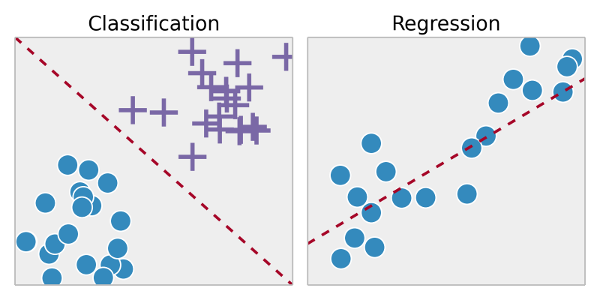
\includegraphics[width=0.7\textwidth]{images/RC.png}
    \caption{Example of classification and regression \citep{rossant2018ipython}.}
  \label{RC}
  
\end{figure}
Classification tasks are mostly known to be discrete, i.e each example belongs to precisely one class, and the set of classes covers the whole possible output space; while as regression tasks are known to be continuous \citep{stephen2009machine}. However there are some overlaps between the algorithms for these tasks. Classification algorithm may predict a continuous value, but the continuous value is in the form of a probability for a class label and a regression algorithm may predict a discrete value, but the discrete value in the form of an integer quantity. Some algorithms can be used for both classification and regression with small modifications, such as decision trees and artificial neural networks \citep{brownlee2013prepare}.  

\subsubsection{Unsupervised learning}

In contrast to labeled data, unlabeled data (i. e., data items without associated labels) can often be obtained in great quantities without much additional effort. The unsupervised learning technique aim at making use of the (additional) information provided by the unlabeled patterns to generate appropriate models. 

As illustrated in Figure \ref{sup-unsup} unsupervised learning where we have only a set observations $T=x_1,x_2,\dots, x_N$. In unsupervised learning we are not interested in prediction, because we do not have an associated output response variable $y_1,y_2,\dots, y_N$. Rather the goal in unsupervised learning algorithms discover interesting information about the measurements on the training set $T$. We look for informative way to visualize the data and interesting patterns among the observations \citep{james2013introduction}. 

\begin{figure}[H]
  \centering
    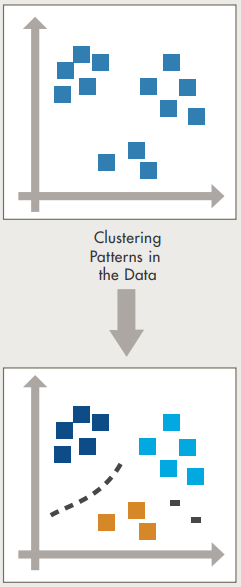
\includegraphics[width=0.35\textwidth]{images/cluster.png}
    \caption{An example of clustering method which reveals hidden patterns in data \citep{Machinelearning}.}
  \label{datagrowth.png}
\end{figure}

Clustering is one of the most commonly used unsupervised method that divides data into clusters. The number of clusters must be initially specified, but since the algorithm converges rapidly, many starting points can be tested. The algorithm uses a distance
criterion for cluster membership, such as the Euclidean distance, and a stopping criterion for iteration, for example, when the cluster membership ceases to change \citep{ball2010data}.

\section{Process of machine learning}
\label{Process}
\subsection{Data preparation}
Machine learning algorithms learn for from data, therefore it is critical that we feed them the right data for the specific problem we want to solve. In this section we will describe the processing steps required for getting data ready for a machine learning algorithm.

There are three steps commonly used in machine learning to process the data, namely data selection, data preprocessing  and data transformation. Data selection has to do with the selection of the the subset of all available data that we need to address the question or problem we are working on. Usually assumptions will be made  about the data and be tested at a later stage. After selecting the data, now come the preprocessing step where we decide how is one going to use the data. Firstly the suitable formatting of the data is considered, could be .csv file format or Numpy file format. In most cases there may be data instances that are incomplete or do not contain useful information. In this case, the removal or fixing of such data is required. When generating the training dataset, it is crucial to also consider the computational cost and memory requirement. Sampling the data by taking smaller representative sample of the selected data that may be much faster for exploring and prototyping solutions before considering the whole dataset can be one of the getaways. The final step is to transform data using either scaling where the preprocessed data may contain attributes with a mixtures of scales for various quantities and is scaled to range between 0 and 1. This helps to stop the weights from getting too large unnecessarily \citep{marsland2015machine}; decompositions which involves attributes that represent a complex concept that may be more useful to a machine learning method when split into the constituent parts, and  aggregations where attributes can be aggregated into a single attribute that would be more meaningful to the problem we are solving \citep{brownlee2013prepare}. The most commonly used scaling methods are referred to as data normalisation, or standardisation \citep{marsland2015machine}.
    
\subsection{Feature engineering}

In machine learning applications, whether it is classification or regression, observation
data that we believe contain information are taken as inputs and fed
to the system for decision making. Some of the goals in these learning algorithms is to achieve the following objectives, i.e improving the prediction performance of the model and reducing the model complexity. This could help reduce the estimation error and thus prevent over fitting. If we  assume that the observation data $\textbf{X}=\mathbb{R}^d$ \citep{shalev2014understanding}, then in most learning algorithms, the complexity depends on the number of
input dimensions, $d$, as well as on the size of the data sample, $N$. 
For reduced memory and computation, we are interested in reducing
the dimensionality of the problem such that we have new feature space $\mathbb{R}^k$ of dimension $k \ll d $. Decreasing $d$ will also decreases the
complexity of the inference algorithm during testing. The
complexity is often broken into two parts: the complexity of training, and the complexity of applying the trained algorithm. Training does not happen very often, and is not usually time critical. However, we often want a decision about a test point quickly, and there are potentially lots of test points when an algorithm is in use, so this needs to have low computational cost \citep{marsland2015machine}.

When data can be explained with fewer features, we get a better idea about the process that underlies the data and this allows knowledge extraction. There are two main methods for reducing dimensionality: feature selection and feature extraction. In feature selection, we are interested in
finding $k$ of the $d$ dimensions that give us the most information and we
discard the other $(d - k)$ dimensions. In feature extraction, we are interested in finding a new set of $k$ dimensions that are combinations of the original d dimensions \citep{alpaydin2014introduction}.
 
During algorithm learning, a feature $x_i\in\mathbb{R}$ become relevant to a target concept $t$ (what is being learned) if there exists a pair of examples A and B in the instance space such that A and B differ only in their assignment to  $x_i$ \citep{blum1997selection}. This implies that twiddling the value of $x_i$ affects the desired output of the learning algorithm. Hence it is important to identifying the features that are most useful for the problem under examination. This invariably requires prior knowledge of the problem and the data. This is process is called feature selection.

In any machine learning, algorithm technique selection is mostly driven by the structure of the dataset and type of the problem one wish to solve (regression or classification). Therefore it is important to have a better understanding of the dataset and which features are useful prior to the selection and splitting of the dataset as described in the previous paragraph. The output of our problem is real number, we therefore categorize our problem as regression. The identified algorithms that are applicable and practical to implement are multi-output regression algorithms to be discussed in more details on the next chapter. 


\section{Tuning model complexity}
\label{comp}
Prediction models, the prediction errors can be decomposed into: error due to bias and error due to variance. There is a tradeoff between a model's ability to minimize bias and variance during training \citep{fortmann2012understanding}. 
\subsection{Bias and variance }
Understanding these two types of error can help us diagnose model results and avoid the mistake of over and under-fitting. understanding the bias and variance will help us to improve the data fitting process resulting in more accurate models \citep{fortmann2012understanding}.
Error due to bias is the difference between the average prediction of our models and the true value which we are trying to predict. i.e. Assume we have multi models built from dataset generated randomly, this will result in the models to have multi predictions, hence the bias measures how far off in general these model's predictions are from the true value. Error due to variance is the variability of a model prediction for a given data point \citep{fortmann2012understanding}. 

\begin{figure}[H]
  \centering
    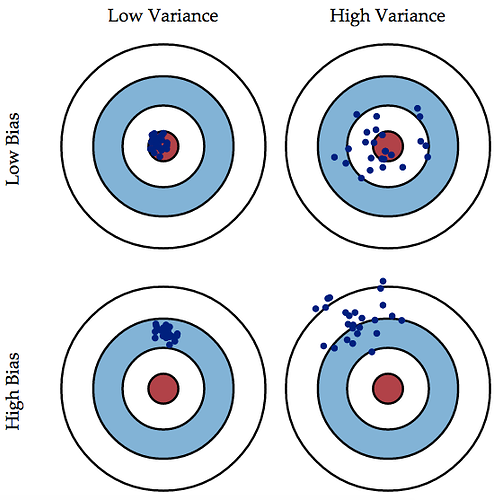
\includegraphics[width=0.48\textwidth]{images/Bias.png}
    \caption{Graphical illustration of bias and variance. The center of each target represents a model that perfectly predicts the true value and as we move away from the centre, our model gets worse in predicting the true value. Variability in training dataset due to outliers or non-standard values will also result in poor prediction \citep{fortmann2012understanding}.}
  \label{RC}
 \end{figure}
 
Suppose  we have a training set $\textbf{X}=\{x_1,\dots x_n\}$ and and a function $\textbf{Y}=f(\textbf{X})+\epsilon$ with $\epsilon$ being an error term normally distributed with zero mean and variance $\sigma^2$. We want to find a function $\widehat{f}(\textbf{X})$  that estimate $f(\textbf{X})$ as well as possible using some learning algorithm technique. In this case, we measure the mean squared prediction error at a point $x$ as :
\begin{align*}
Err(x)&= \mathbb{E}\left[(\textbf{Y}- \widehat{f}(x) ) \right]\\
&= \mathbb{E}\left[ \textbf{Y}^2 +\widehat{f}(\textbf{x})^2 -2\textbf{Y}\widehat{f}(x)\right]\\
&= \mathbb{E}\left[\textbf{Y}^2 \right] + \mathbb{E}\left[\widehat{f}(x)^2 \right]- 2\mathbb{E}\left[\textbf{Y}\widehat{f}(x)\right]
\end{align*}
Since $\text{Var}(\textbf{Y}) = \mathbb{E}\left[\textbf{Y}^2 \right]- \mathbb{E}\left[\textbf{Y}\right]^2$, then we have  $\mathbb{E}\left[\textbf{Y}^2 \right] =\text{Var}(\textbf{Y}) + \mathbb{E}\left[\textbf{Y}\right]^2$, such that
\begin{align*}
Err(x)&= \text{Var}(\textbf{Y}) + \mathbb{E}\left[\textbf{Y}\right]^2 + \text{Var}\left[\widehat{f}(x)\right] + \mathbb{E}\left[\widehat{f}(x) \right]^2- 2f\mathbb{E}\left[\widehat{f}(x) \right]\\
&= \text{Var}(\textbf{Y}) + \text{Var}(\widehat{f}) + (f(x)- \mathbb{E}\left[
\widehat{f}\right]^2)\\
&= \sigma^2 + \text{Var}(\widehat{f})+ \text{Bias}\left[\widehat{f}\right]^2
\end{align*}

where $\sigma^2$ represents the irreducible error. 

There are various ways of managing the bias and variance during training, one of them being the bagging  and resampling. These techniques can be used to reduce the variance in model prediction. In bagging (Bootstrap Aggregating), replicates of the original data set are created using random selection with replacement. Each randomly selected data set is then used to construct a new model and the models are gathered together into an ensemble. To make a prediction, all of the models in the ensemble are polled and their results are averaged.

\subsection{Over fitting and under fitting}

\begin{figure}[H]
  \centering
    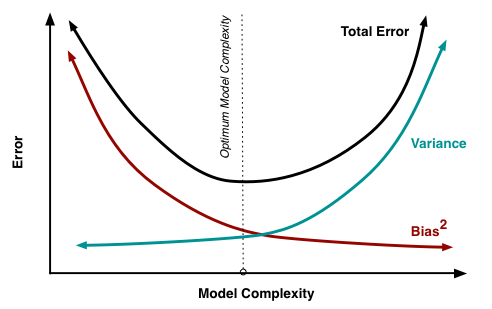
\includegraphics[width=0.7\textwidth]{images/biasvariance.png}
    \caption{The bias and variance contributing to total error. Dealing with bias and variance is about dealing with over-fitting and under-fitting. The bias is reduced and the variance is increased in relation to the model complexity. As more parameters are added to a model, the complexity of the model increases and variance becomes our primary concern while bias steadily decreases \citep{fortmann2012understanding}.}  
\end{figure}

Understanding bias and variance is critical for understanding the behaviour of prediction models, but in general what we really care about is the overall error $Err$, not the specific decomposition. The sweet spot for any model is the level of complexity at which the increase in bias is equivalent to the reduction in variance. If our model complexity exceeds this sweet spot, we are in effect over-fitting our model; while if our complexity falls short of the sweet spot, we are under-fitting the model \citep{fortmann2012understanding}.









